\documentclass[runningheads]{llncs}

\usepackage[T1]{fontenc}
\usepackage{graphicx}
\usepackage{amssymb,amsmath}
\usepackage{siunitx}
\usepackage{booktabs}
\usepackage[hidelinks]{hyperref}

\title{Supplementary Material:\\
Low-Magnification SEM Suffices: Interpretable Deep Learning
for Multi-Scale Fracture-Cause Classification in
Zirconia-Toughened Alumina}
\titlerunning{Supplementary Material}
\author{Julian Schmid \and Pawel Astankow \and Tom Vater \and
        Julius Beck \and Robert Cichon \and Danny Krautz}
\authorrunning{J. Schmid et al.}
\institute{CeramTec GmbH, Plochingen, Germany}

% Reset numbering: S1, S2, ... statt 1, 2, ...
\renewcommand{\thetable}{S\arabic{table}}
\renewcommand{\thefigure}{S\arabic{figure}}

\begin{document}
\maketitle

\noindent This document accompanies the paper
``Low-Magnification SEM Suffices...'' and provides additional
details on the hyperparameter search, optimal configuration,
per-fold metrics, and learning curves.

% =============== HIER deine Tabellen 1:1 reinpasten ===============



% ---------------------------------------------------------------
%                         Supplement
% ---------------------------------------------------------------

\appendix
\section*{Supplementary Material}

\begin{table}[h]
    \centering
    \caption{Optimal hyperparameter configuration found for the ViT model.}
    \setlength{\tabcolsep}{4pt}      % default ist 6pt

    \label{tab:vit_best_trial}
    \begin{tabular}{@{}ll@{}}
    \toprule
    \textbf{Parameter} & \textbf{Value} \\
    \midrule
    Learning Rate        & \num{7.3e-5} \\
    Weight Decay         & 0.140 \\
    Drop Path Rate       & 0.10 \\
    Label Smoothing      & 0.00 \\
    Warm-up Steps        & 103 \\
    Layer-wise LR Decay  & 0.843 \\
    RandAugment: \#Ops   & 2 \\
    RandAugment: Magnitude & 12 \\
    Patch Drop Rate      & 0.111 \\
    \bottomrule
    \end{tabular}
\end{table}

\begin{table}[h]
    \centering
    \setlength{\tabcolsep}{4pt}      % default ist 6pt
    \caption{Training and validation metrics (mean ± std over 5 folds).}
    \label{tab:supp_metrics}
    \resizebox{\linewidth}{!}{%
    \begin{tabular}{lcccc}
        \toprule
        Metric & Train Mean ± SD & Val Mean ± SD & Train CI & Val CI \\
        \midrule
        Accuracy   & 0.998 ± 0.001 & 0.907 ± 0.008 & [0.997, 0.999] & [0.897, 0.917] \\
        Macro-F$_1$& 0.998 ± 0.001 & 0.888 ± 0.017 & [0.997, 0.999] & [0.867, 0.909] \\
        Precision  & 0.998 ± 0.001 & 0.917 ± 0.010 & [0.997, 0.999] & [0.905, 0.929] \\
        Recall     & 0.998 ± 0.001 & 0.866 ± 0.025 & [0.997, 0.999] & [0.835, 0.897] \\
        \bottomrule
    \end{tabular}%
    }
\end{table}

\begin{figure}[h]
    \centering
    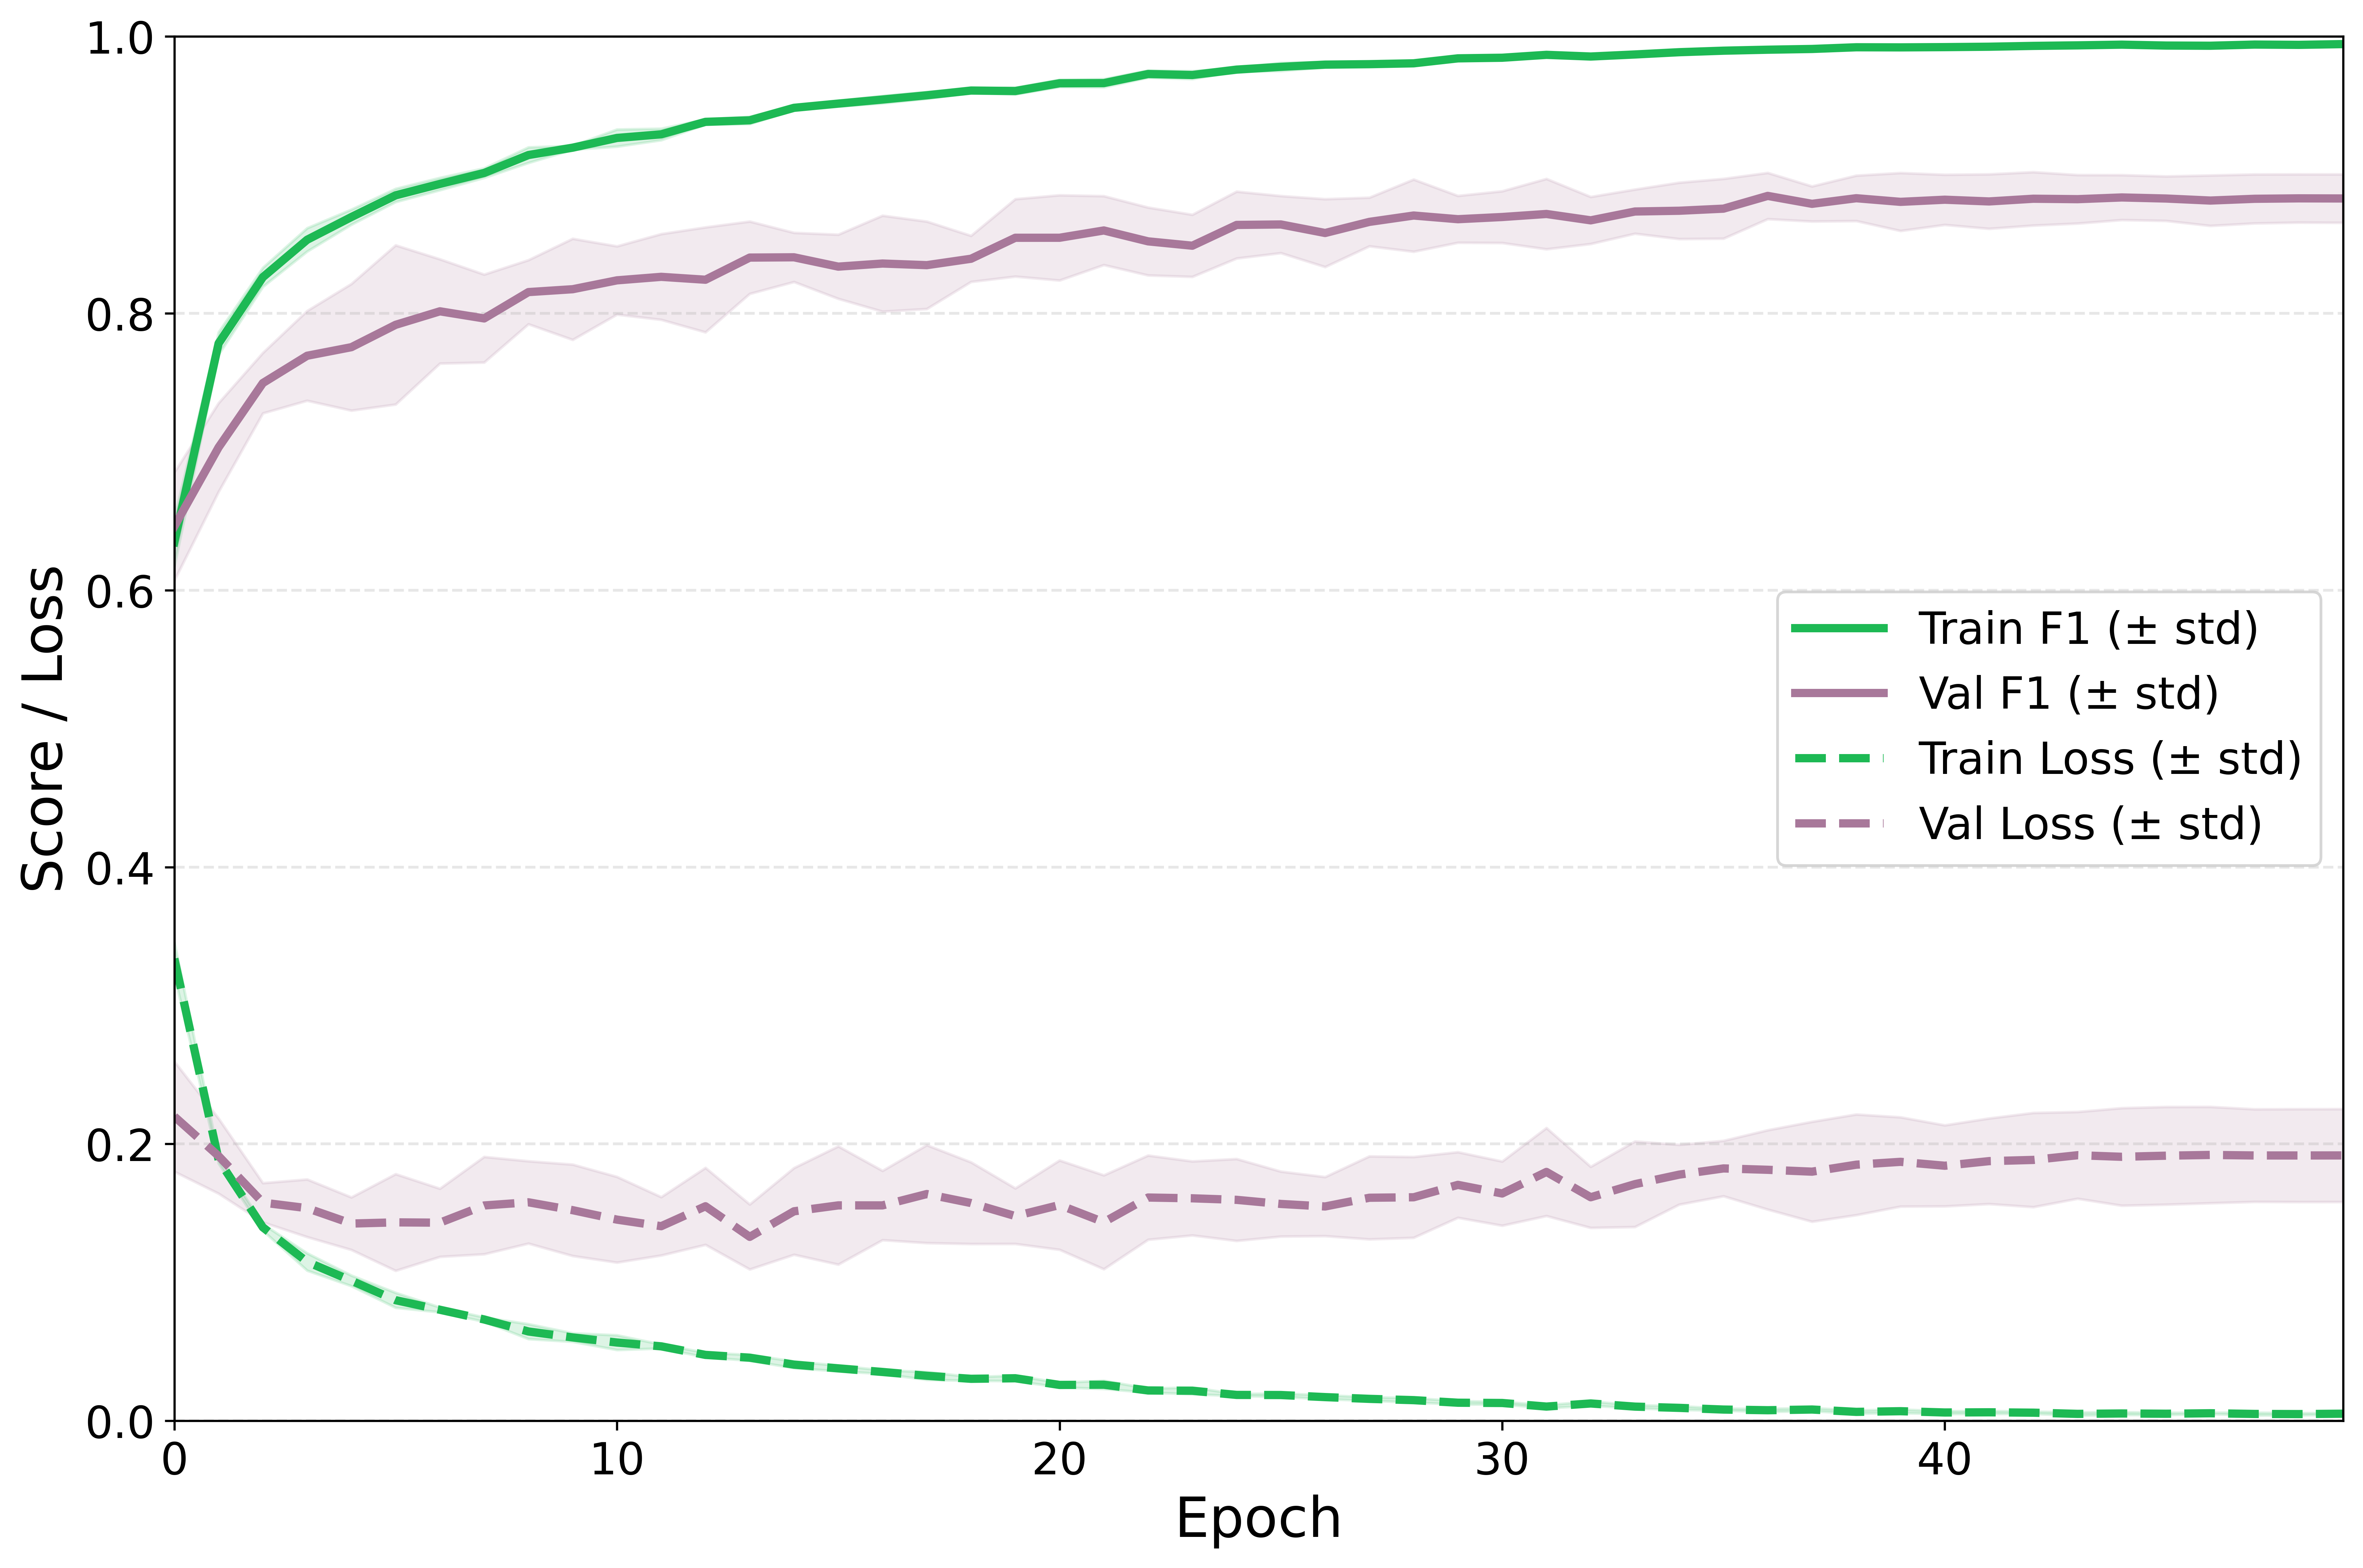
\includegraphics[width=0.75\linewidth]{curves.png}
    \caption{Training and validation curves for macro-F$_1$ and loss across 50~epochs (mean ± std over 5 folds).}
    \label{fig:supp_learning_curves}
\end{figure}



\begin{table}[!t!]
  \centering
  \caption{ViT hyperparameter search space explored with Optuna.}
  \label{tab:vit_hpo_params}
  \begin{tabular}{@{}lll@{}}
  \toprule
  \textbf{Parameter} & \textbf{Range / Options} & \textbf{Type} \\
  \midrule
  Learning Rate      & $10^{-6}$ – $10^{-4}$ (log) & Continuous \\
  Weight Decay       & 0.0 – 0.3                   & Continuous \\
  Drop Path Rate     & \{0.0, 0.1, 0.2\}           & Categorical \\
  Label Smoothing    & \{0.0, 0.05, 0.1\}          & Categorical \\
  Warm-up Steps      & 50 – 500                    & Integer \\
  Layer-wise LR Decay& 0.6 – 1.0                   & Continuous \\
  RandAugment Ops    & 1 – 3                       & Integer \\
  RandAugment Magnitude & 5 – 15                   & Integer \\
  Patch Drop Rate    & 0.0 – 0.2                   & Continuous \\
  \bottomrule
  \end{tabular}
\end{table}

\end{document}
